\documentclass[10pt,a4paper]{article}
\usepackage[pdftex]{graphicx}
\usepackage{graphicx}
\usepackage{amsmath}
\usepackage{listings}
\usepackage{url}
\usepackage{amsmath}
\usepackage[left=20mm, top=0in]{geometry}
\date{}
\begin{document}
\title{Assignment No 6}
\author{JAGAN M J EE20B047}
\maketitle


\section{AIM}

Aim is to explore the use of Python libraries in analysing Linear Time-Invariant systems

\section{Time response of a spring system}
We need to find the time response of a spring system given by the equation 

$$ \ddot{x} + 2.25x = f(t)  $$

where f(t) is given by \\

f(t) = cos{(1.5t)}exp(-0.5t)u(t) \\

and its laplace transform is given by :
\[
    F(s) = \frac{s+0.5}{s^2 + s + 2.5}
\]

On solving in the laplace domain, we get 
\[
    X(s) = \frac{s+0.5}{(s^2 + s + 2.5)(s^2 + 2.25)}
\]

A graph is plotted between x(t) and t for t from 0 to 50 sec as shown below :

\begin{figure}[!tbh]

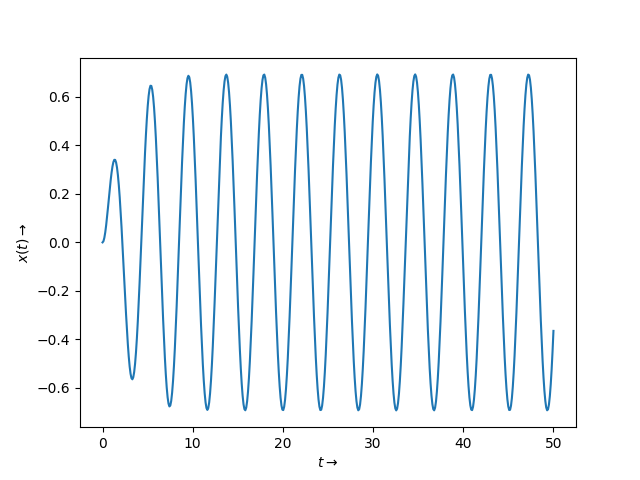
\includegraphics[width = 0.9\textwidth]{1.png}
\caption{Time response of a spring}

\end{figure}

For a smaller decay of 0.05, we get the following plot: \\

\begin{figure}[!tbh]

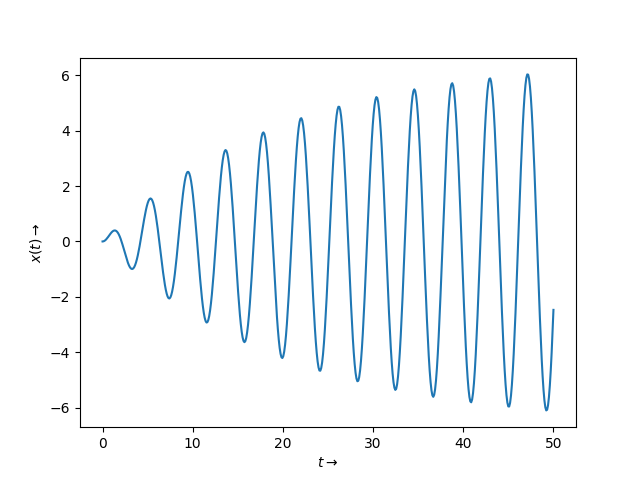
\includegraphics[width = 0.9\textwidth]{2.png}
\caption{Time response of a spring with smaller decay}

\end{figure}

\section{Response over different frequencies}

The following graphs are obtained by varying the frequency of the force f(t)

\begin{figure}[!tbh]

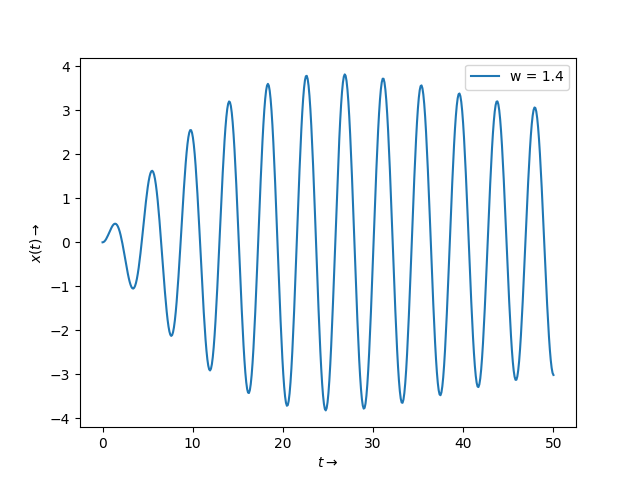
\includegraphics[width = 0.9\textwidth]{3a.png}

\end{figure}

\begin{figure}[!tbh]

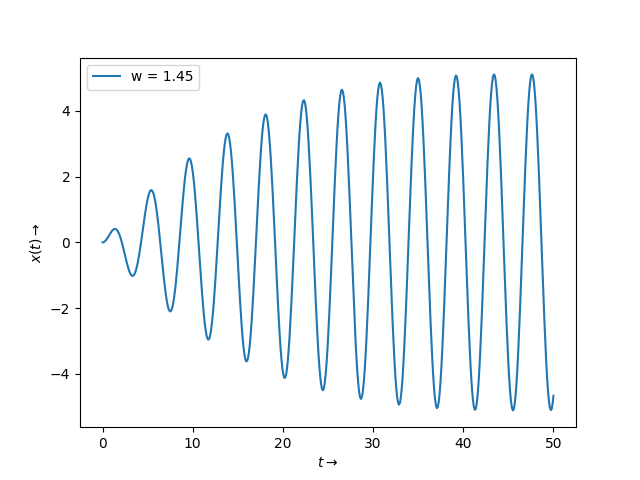
\includegraphics[width = 0.9\textwidth]{3b.png}

\end{figure}

\begin{figure}[!tbh]

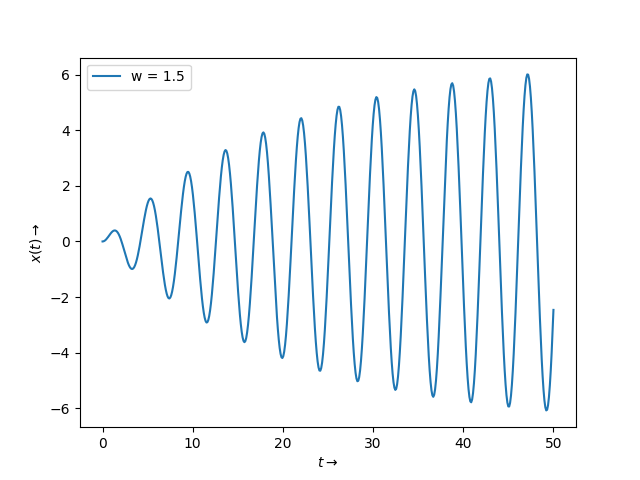
\includegraphics[width = 0.9\textwidth]{3c.png}

\end{figure}

\begin{figure}[!tbh]

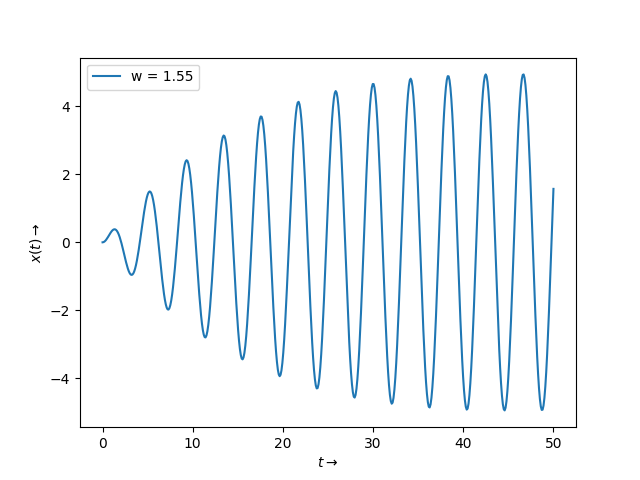
\includegraphics[width = 0.9\textwidth]{3d.png}

\end{figure}

\begin{figure}[!tbh]

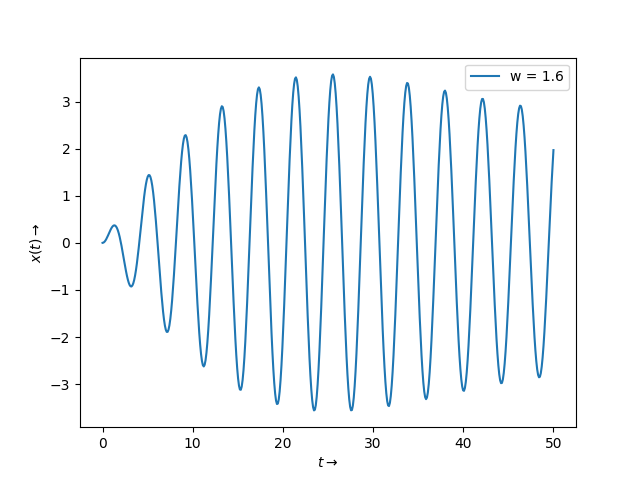
\includegraphics[width = 0.9\textwidth]{3e.png}

\end{figure}

From the given equation, we se that the natural response of the system has the frequency w = 1.5 rad/s. That is, maximum amplitude of the oscilaation is obtained when the frequency of f(t) is 1.5 rad/s, as in case of resonance\\ \\ \\ \\ \\ \\ \\ \\ \\ \\ \\ \\ \\ \\ \\ \\ \\ \\ \\ \\ \\ \\ \\ \\ \\ \\ \\ \\ \\ \\ \\ \\ \\ \\ \\ \\ 

\section{The coupled spring problem}

The coupled equation are : 

$$ \ddot{x} + (x - y) = 0  $$
$$ \ddot{y} + 2(y - x) = 0  $$

On Solving the equation, we get : 

$$ \ddddot{x} + 3\ddot{x} = 0  $$

By taking the Laplace transform of this equation, we get : 

\[
    X(s) = \frac{s^2+2}{s^3 + 3s}
\]

Similarly for y equation we get, 

$$ \ddddot{y} + 3\ddot{y} = 0  $$

By taking the Laplace transform of this equation, we get : 

\[
    Y(s) = \frac{2}{s^3 + 3s}
\]

The following plots are obtained for x(t) and y(t) for t between 0 and 20s :\\
We observe that x(t) and y(t) are sinusoids of the same frequency, but with different amplitude and phase\\ \\ \\ \\ \\ \\ \\ \\ \\ \\ \\ \\ \\ \\ 

\begin{figure}[!tbh]

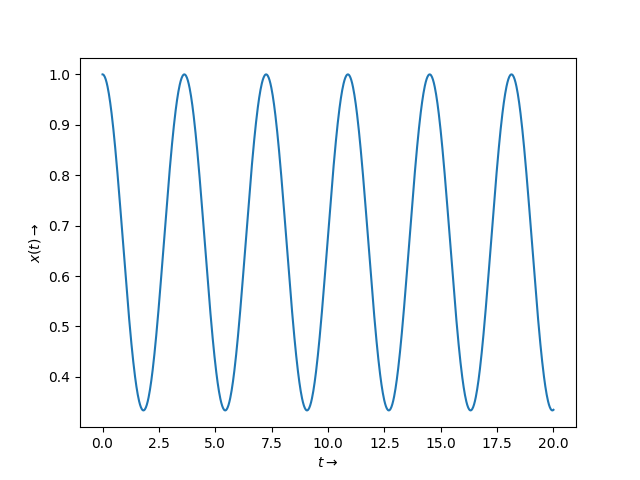
\includegraphics[width = 0.9\textwidth]{4a.png}
\caption{Solution for x(t)}

\end{figure}

\begin{figure}[!tbh]

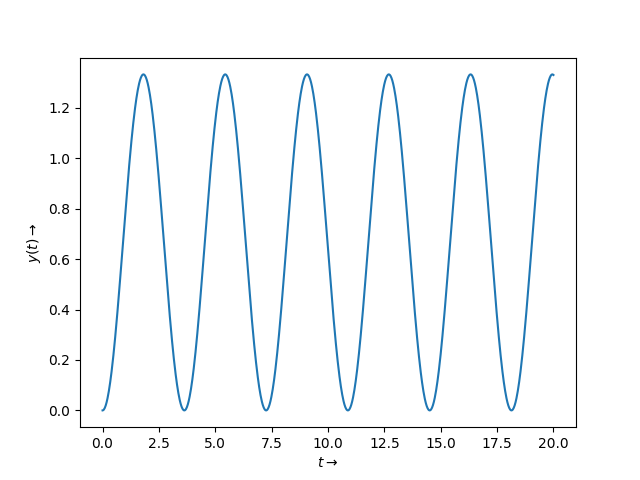
\includegraphics[width = 0.9\textwidth]{4b.png}
\caption{Solution for y(t)}

\end{figure}

\section{The Two-Port Network}

The Steady-State transfer function of the given circuit is given by :

\[
    H(s) = \frac{10^6}{s^2 + 100s + 10^6}
\]

The magnitude and phase response is given below : 

\begin{figure}[!tbh]

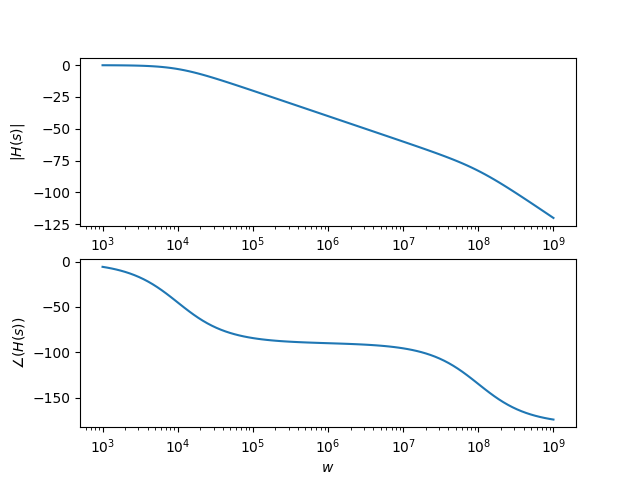
\includegraphics[width = 0.9\textwidth]{5.png}
\caption{Magnitude and phase plot of H(s)}

\end{figure}

Now, when the input to this system is 

\[Vi(t) = \cos{(10^3t)}-\cos{(10^6t)} \]

The output is given by : 
 
\[ Vo(s) = Vi(s)H(s) \]

A graph is plotted for Vo(t) v/s t where t is from 0 to 30us : 

\begin{figure}[!tbh]

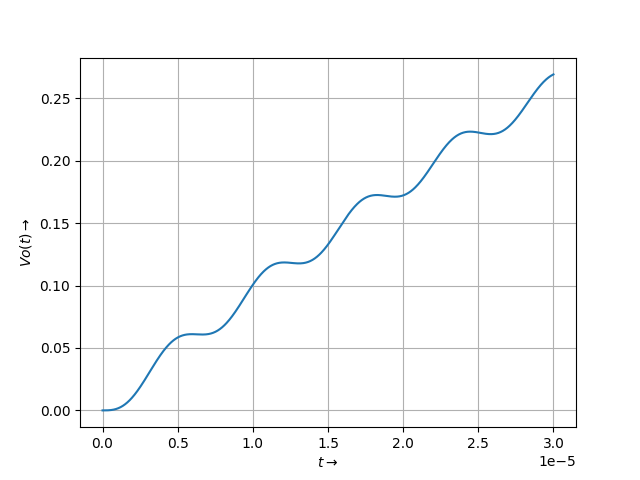
\includegraphics[width = 0.9\textwidth]{6.png}
\caption{Vo(t) v/s t}

\end{figure}

These variations are determined by the high frequency component of v(t)\\ \\ \\ \\ \\ \\ \\ \\ \\ \\ \\ \\  \\ \\ \\ \\ \\
 
On plotting for t from 0 to 10ms : 

\begin{figure}[!tbh]

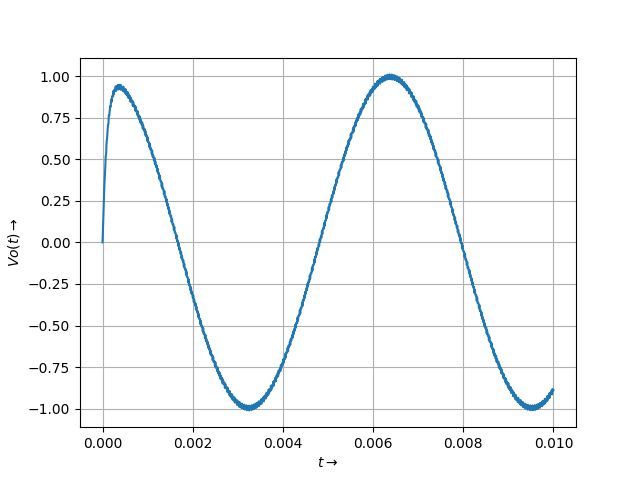
\includegraphics[width = 0.9\textwidth]{7.png}
\caption{Vo(t) v/s t}

\end{figure}

From the Bode plot of H(s) , we notice that system provides unity gain at a low frequency of 1000 rad/s. Thus, low frequency component is more preserved in the output. The system dampens a high frequency of 1000000 rad/s which shows that nature of the circuit is to act as a low pass filter circuit


\section{Conclusion}

The scipy.signal library provides a useful toolkit of functions for circuit analysis. The toolkit was used for the analysis of LTI systems in various domains. The forced response of a simple spring body system was obtained over various frequencies of the applied force, and highest amplitude was observed at resonant frequency. A coupled spring problem was solved using the sp.impulse function to obtain two sinusoids of the same fequency. A two port network, functioning as a low pass filter was analysed and the output was obtained for a mixed frequency input.

\end{document}